\documentclass{standalone}
\usepackage{tikz}
\usetikzlibrary{backgrounds}
\usetikzlibrary{decorations.pathmorphing}
\usepackage{xcolor}

\tikzset{snake it/.style={decorate, decoration=snake}}


\definecolor{plotblue}{RGB}{100,100,255}
%\definecolor{myblue}{RGB}{8,164,214}
\definecolor{myred}{RGB}{143,42,41}
\definecolor{forestgreen}{RGB}{34,139,34}
\definecolor{highdive}{RGB}{10,169,194}
\definecolor{charcoal}{RGB}{74,74,74}

\begin{document}
	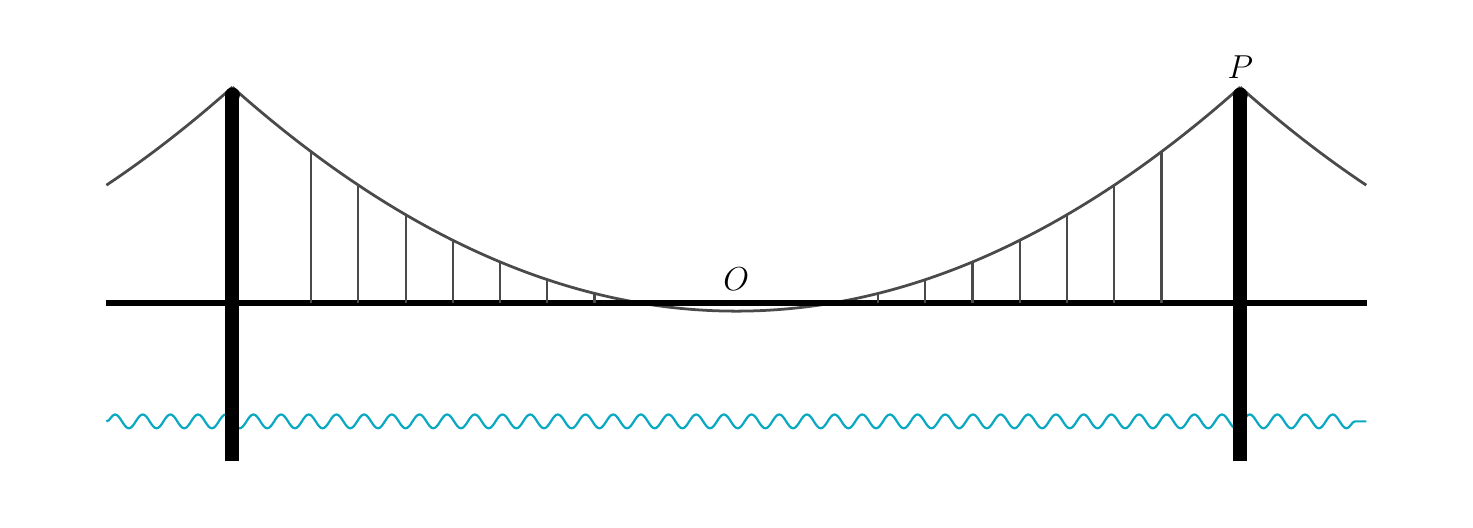
\begin{tikzpicture}[cross/.style={draw, cross out, minimum size=2*(#1-1pt), inner sep=0pt, outer sep=0pt}, x=1mm, y=1mm,
		>=latex,   %Voreinstellung für Pfeilspitzen
		font= \footnotesize, scale=1]
		\begin{scope}[on background layer]
			\fill[white] (-90,-25) rectangle (90,35);
		\end{scope}
		%Funktionen zeichnen:
		\clip(-90,-25) rectangle (90,35); %Bildbereich
		\draw[charcoal,line width=1pt,domain=-64:64,samples=2000] plot (\x, {(\x)^2/144-1)}); %Parabel
		\draw[charcoal,line width=1pt,domain=-80:-64,samples=2000] plot (\x, {(\x+128)^2/144-1)}); %Parabel
		\draw[charcoal,line width=1pt,domain=64:80,samples=2000] plot (\x, {(\x-128)^2/144-1)}); %Parabel
		\draw[black,line width=2pt,domain=-80:80,samples=2000] plot (\x, {0}); %Fahrbahn
		\path [draw=highdive,thick,snake it] (-80,-15) -- (80,-15); %Meeresspiegel
		\draw[black,line width=5pt] (-64,-20) -- (-64,238/9); %linker Pfosten
		\draw[fill=black] (-64,238/9) circle (2.5pt);
		\draw[black,line width=5pt] (64,-20) -- (64,238/9); %rechter Pfosten
		\draw[fill=black] (64,238/9) circle (2.5pt);
		\foreach \x in {-54,-48,-42,-36,-30,-24,-18,18,24,30,36,42,48,54} \draw[charcoal,thick] (\x,0) -- (\x,{(\x)^2/144-1)}); %Aufhängung
		%Beschriftung
		\node[black]  at (0,3) {\large$O$};
		\node[black]  at (64,30) {\large$P$};
	\end{tikzpicture}


\end{document}